\documentclass[twocolumn]{article}
\usepackage[margin=0.75cm]{geometry}
\usepackage{hyperref}
\hypersetup{
    colorlinks,
    citecolor=blue,
    filecolor=blue,
    linkcolor=blue,
    urlcolor=blue
}

\usepackage{graphicx, wrapfig, caption, multirow, mathtools, amsfonts, booktabs, siunitx, accents, circuitikz, pgfplots}
\setlength{\columnseprule}{.75pt}
\def\columnseprulecolor{\color{black}}
\newcommand{\overbar}[1]{\mkern 1.5mu\overline{\mkern-1.5mu#1\mkern-1.5mu}\mkern 1.5mu}

\setlength{\parindent}{0pt}
\setlength{\parskip}{6pt}

\everymath{\displaystyle}

\title{
	\vspace{-2em}
	\normalsize \textbf{ECE 203 Formula Sheet} \\
	\small Eddie Guo \\
	\dotfill
	\vspace{-5em}
}
\date{}

\begin{document}
\maketitle

\small

\textbf{Review}

\begin{minipage}{0.39\columnwidth}
    \begin{circuitikz}[american, scale=1.5]
        \ctikzset{bipoles/length=9mm}
        \draw (0,-1)
        to [short] (1, -1)
        to [R=$R_1$, i^<=$I_1$] (1, 0)
        to [short] (0, 0);
        \draw (1,-1)
        to [short] (2, -1)
        to [R=$R_2$, i^<=$I_2$] (2, 0)
        to [short] (1, 0);
        \draw (0,-1)
        to [I, l=\mbox{$I$}] (0, 0);
    \end{circuitikz}
\end{minipage}
\hfill
\begin{minipage}{0.6\columnwidth}
    \centering
    \textit{Current division} \\[.5em]
    $I_1 = \frac{R_2}{R_1 + R_2} I$
\end{minipage}

\begin{minipage}{0.39\columnwidth}
    \begin{circuitikz}[american, scale=1.5]
        \ctikzset{bipoles/length=9mm}
        \draw (0,-1)
        to [V, l=\mbox{$V$}, invert] (0,0)
        to [R=$R_1$, v>=$V_1$] (1, 0)
        to [R=$R_2$] (1, -1)
        to [short] (0, -1);
    \end{circuitikz}
\end{minipage}
\hfill
\begin{minipage}{0.6\columnwidth}
    \centering
    \textit{Voltage division} \\[.5em]
    $V_1 = \frac{R_1}{R_1 + R_2} V$
\end{minipage}

\dotfill

\textbf{Capacitors and Inductors}

$q(t) = Cv(t)$ \hfill $i_c(t) = C \frac{dv(t)}{dt}$ \hfill $v_c(t) = v_c(t_0) + \frac{1}{C} \int_{t_0}^t i_c(x)\ dx$

$p_c(t) = v_c(t) i_c(t)$ \hfill $E_c(t) = \frac{1}{2} CV^2 = \frac{Q^2}{2C} = \frac{1}{2} QV$

$L = \frac{\lambda(t)}{i_L(t)}$ \hfill $v_L(t) = L \frac{di(t)}{dt}$ \hfill $i_L(t) = i_L(t_0) + \frac{1}{L} \int_{t_0}^t i_L(x)\ dx$

$p_L(t) = v_L(t) i_L(t)$ \hfill $E_L(t) = \frac{1}{2} L [i_L(t)]^2$

$C_s = \left( \sum_{i=1}^N \frac{1}{C_i} \right)^{-1}$ \hfill $C_p = \sum_{i=1}^N C_i$ \hfill $L_s = \sum_{i=1}^N L_i$ \hfill $L_p = \left( \sum_{i=1}^N \frac{1}{L_i} \right)^{-1}$

\dotfill

\textbf{General Solution of First-Order Circuits}

$\dot{x}(t) + ax(t) = A$, where $x(t) = K_1 + K_2 e^{-t/\tau}$

$\quad K_1 = \frac{A}{a}$ \hfill $\tau = \frac{1}{a}$ \hfill $K_2 = x(0) - K_1$

$\quad v(t) = v(\infty) + [v(0) - v(\infty)] e^{-t/\tau}$ \hfill $\quad i(t) = i(\infty) + [i(0) - i(\infty)] e^{-t/\tau}$

Compute $R_{\text{Th}}$ from view of energy storage device to find $\tau$.

\vspace{-.5em}
\dotfill

\textbf{Transient Behaviour of First-Order Circuits}

% RL
\textit{Discharging RL Circuit} \\
\begin{minipage}{0.34\columnwidth}
    \begin{circuitikz}[american, scale=1.5]
        \ctikzset{bipoles/length=9mm}
        \draw (0,0)
        to[R=$R$, v<=$v(t)$] (0,1)
        to[short] (1,1)
        to[L=$L$] (1,0)
        to[short] (0, 0);
\end{circuitikz}
\end{minipage}
\hfill
\begin{minipage}{0.64\columnwidth}
    $L \frac{di(t)}{dt} + Ri(t) = 0$ \hfill $\quad v_c(0^-) = v_c(0^+)$ \\[.5em]
    $i(t) = i(0^+) e^{-t/\tau}$ \hfill $\tau = L/R$ \\[.5em]
    $E_L(0^+) = \frac{1}{2} L \left( \frac{V_s}{R} \right)^2$ \hfill $E_L(\infty) = 0$ \\[.5em]
\end{minipage}

% RC
\textit{Discharging RC Circuit} \\
\begin{minipage}{0.34\columnwidth}
    \begin{circuitikz}[american, scale=1.5]
        \ctikzset{bipoles/length=9mm}
        \draw (0,0)
        to[R=$R$, v<=$v(t)$] (0,1)
        to[short] (1,1)
        to[C=$C$] (1,0)
        to[short] (0, 0);
\end{circuitikz}
\end{minipage}
\hfill
\begin{minipage}{0.64\columnwidth}
    $C \frac{dv(t)}{dt} + \frac{v(t)}{R} = 0$ \hfill $i_L(0^-) = i_L(0^+)$ \\[.5em]
    $v(t) = v(0^+) e^{-t/\tau}$ \hfill $\tau = RC$ \\[.5em]
    $E_C(0^+) = \frac{1}{2} Cv(0^+)$ \hfill $E_C(\infty) = 0$
\end{minipage}

\dotfill

\textbf{Step Response of First-Order Circuits}

% VRL
\textit{Charging RL Circuit} \\
\begin{minipage}{0.34\columnwidth}
    \begin{circuitikz}[american, scale=1.5]
        \ctikzset{bipoles/length=9mm}
        \draw (0,0)
        to[V=$V_s$, invert] (0,1)
        to[R=$R$, v>=$v(t)$] (1,1)
        to[L=$L$, i>=$i(t)$] (1,0)
        to[short] (0, 0);
\end{circuitikz}
\end{minipage}
\hfill
\begin{minipage}{0.64\columnwidth}
    $L \frac{di(t)}{dt} + Ri(t) = V_s$ \\[.5em]
    $i(t) = \frac{V_s}{R} \left(1 - e^{-t/\tau} \right)$ \hfill $\tau = L/R$ \\[.5em]
    $v_L(t) = V_s e^{-t/\tau}$
\end{minipage}


\newpage


% VRC
\textit{Charging RC Circuit} \\
\begin{minipage}{0.34\columnwidth}
    \begin{circuitikz}[american, scale=1.5]
        \ctikzset{bipoles/length=9mm}
        \draw (0,0)
        to[V=$V_s$, invert] (0,1)
        to[R=$R$, v>=$v(t)$] (1,1)
        to[C=$C$, i>=$i(t)$] (1,0)
        to[short] (0, 0);
    \end{circuitikz}
\end{minipage}
%
\begin{minipage}{0.64\columnwidth}
    $C \frac{dv(t)}{dt} + \frac{v(t) - V_s}{R} = 0$ \\[.5em]
    $i(t) = \frac{V_s}{R} \left(1 - e^{-t/\tau} \right)$ \hfill $\tau = RC$ \\[.5em]
    $v(t) = V_s \left( 1 - e^{-t/\tau} \right)$
\end{minipage}

\dotfill

\textbf{General Solution of Second-Order Circuits}

$\ddot{x}(t) + a_1 \dot{x}(t) + a_2 x(t) = A$, where $x(t) = x_p(t) + x_c(t)$

$\quad x_p(t) = \frac{A}{a_2}$ \hfill $x_c(t) = K_1 e^{s_1 t} + K_2 e^{s_2 t}$

$\quad x(0) = \frac{A}{a_2} + K_1 + K_2$ \hfill $\dot{x}(0) = K_1 s_1 + K_2 s_2$

$\quad$Obtain $\dot{x}(0)$ from ODE of circuit

$ \text{Characteristic eq: } s^2 + 2 \zeta \omega_0 s + \omega_0^2 = 0$

$\quad \zeta > 1:\ x_c(t) = K_1 e^{-\omega_0 (\zeta - \sqrt{\zeta^2 - 1}) t} + K_2 e^{-\omega_0 (\zeta + \sqrt{\zeta^2 - 1}) t}$

$\quad \zeta = 1:\ x_c(t) = (B_1 + B_2 t) e^{-\zeta \omega_0 t}$

$\quad \zeta < 1:\ x_c(t) = e^{-\sigma t} (A_1 \cos \omega_d t + A_2 \sin \omega_d t)$

$\quad\quad \sigma = \omega_0 \zeta, \quad \omega_d = \omega_0 \sqrt{1 - \zeta^2}$

\vspace{-.5em}
\dotfill

\textbf{Second-Order Circuit w/o Source}

\textit{Parallel RLC Circuit}

\begin{minipage}{0.44\columnwidth}
\begin{circuitikz}[american, scale=1.5]
    \ctikzset{bipoles/length=9mm}
    \draw (0,0)
    to [short] (0, 0)
    to [R, a=$R$, v^=$v(t)$] (0, -1);
    \draw (0, 0)
    to [short] (1, 0)
    to [L=$L$] (1, -1)
    to [short] (0, -1);
    \draw (1, 0)
    to [short] (2, 0)
    to [C=$C$, i>=$i_c(t)$] (2, -1)
    to [short] (1, -1);
\end{circuitikz}
\end{minipage}
\hfill
\begin{minipage}{0.55\columnwidth}
    $v(0) = K_1 + K_2$ \\[0.5em]
    $\frac{dv(0)}{dt} = \frac{1}{C} i_c(t) = K_1 s_1 + K_2 s_2$ \\[0.5em]
    $\frac{d^2 v_c(t)}{dt^2} + \frac{1}{RC} \frac{dv_c(t)}{dt} + \frac{1}{LC} v_c(t) = 0$
\end{minipage}

\textit{Series RLC Circuit}

\begin{minipage}{0.44\columnwidth}
    \begin{circuitikz}[american, scale=1.5]
        \ctikzset{bipoles/length=9mm}
        \draw (0,-1)
        to [R=$R$] (0, 0)
        to [L=$L$, i>=$i(t)$] (2, 0)
        to [C=$C$] (2, -1)
        to [short] (0, -1);
    \end{circuitikz}
\end{minipage}
\hfill
\begin{minipage}{0.55\columnwidth}
    $i(0) = K_1 + K_2$ \\[0.5em]
    $\frac{di(0)}{dt} = \frac{v_L(0)}{L} = K_1 s_1 + K_2 s_2$ \\[0.5em]
    $\frac{d^2 i_L(t)}{dt^2} + \frac{R}{L} \frac{di_L(t)}{dt} + \frac{1}{LC} i_L(t) = 0$
\end{minipage} \vspace{-.5em}

\dotfill

\textbf{Second-Order w/ Source}

% IRLC
\textit{Parallel RLC Circuit with Current Source}

\begin{circuitikz}[american, scale=1.5]
    \ctikzset{bipoles/length=9mm}
    \draw (0,-1)
    to [I, l=\mbox{$i_s(t)$}] (0,0)
    to [short] (1, 0)
    to [R, a=$R$, v^=$v_c(t)$] (1, -1)
    to [short] (0, -1);
    \draw (1, 0)
    to [short] (2, 0)
    to [C=$C$] (2, -1)
    to [short] (1, -1);
    \draw (2, 0)
    to [short] (3, 0)
    to [L=$L$, i>=$i(t)$] (3, -1)
    to [short] (2, -1);
\end{circuitikz}

$\frac{d^2 v_c(t)}{dt^2} + \frac{1}{RC} \frac{dv_c(t)}{dt} + \frac{1}{LC} v_c(t) = \frac{1}{C} \frac{di_s(t)}{dt}$

\vspace{1em}

\textit{Series RLC Circuit with Voltage Source}

\begin{circuitikz}[american, scale=1.5]
    \ctikzset{bipoles/length=9mm}
    \draw (0,-1)
    to [V=$v_s(t)$, invert] (0, 0)
    to [R=$R$] (1, 0)
    to [C=$C$, v=$v(t)$] (2, 0)
    to [L=$L$, i>=$i_L(t)$] (2, -1)
    to [short] (0, -1);
\end{circuitikz}

$\frac{d^2 i_L(t)}{dt^2} + \frac{R}{L} \frac{di_L(t)}{dt} + \frac{1}{LC} i_L(t) = \frac{1}{L} \frac{dv_s(t)}{dt}$


\cleardoublepage

\textbf{Tricky Questions}

\begin{minipage}{0.49\columnwidth}
    \textit{Set up the 2nd-order eq for $v_c(t)$.} \\[.5em]
    $8 = i_L(t) + i_R(t)$ \\[0.5em]
    $\implies i_R(t) = 8 - i_L(t)$ \\[0.5em]
    $L \frac{di_L(t)}{dt} + v_c(t) - R(8 - i_L(t)) = 0$

    $\quad\quad$But $i_L(t) = i_c(t) = C \frac{dv_c(t)}{dt}$
\end{minipage}
\hfill
\begin{minipage}{0.49\columnwidth}
\flushright
\begin{circuitikz}[american, scale=1.35]
    \ctikzset{bipoles/length=9mm}
    \draw (0,-2)
    to [I, l=\mbox{8 A}] (0, 0)
    to [short] (2, 0);
    \draw (1, 0)
    to [L=$L$, i=$i_L(t)$] (1, -1)
    to [C=$C$, v=$v_c(t)$] (1, -2)
    to [short] (0, -2);
    \draw (2, 0)
    to [R=$R$, i=$i_R(t)$] (2, -2)
    to [short] (1, -2);
\end{circuitikz}
\end{minipage}

Therefore, $LC \frac{d^2 v_c(t)}{dt^2} + v_c(t) + RC \frac{dv_c(t)}{dt} = 8R$

\dotfill

\textit{Which circuits do not violate any $v$-$i$ terminal relationships?}

\begin{circuitikz}[american, scale=1.35]
    \ctikzset{bipoles/length=9mm}
    \draw (0, -1)
    to [I, l=\mbox{$Iu(t)$}] (0, 0)
    to [short] (0.5, 0)
    to [L] (0.5, -1)
    to [short] (0, -1);
    \node at (0.25, -1.25) {Not allowed};
\end{circuitikz}
\hfill
\begin{circuitikz}[american, scale=1.35]
    \ctikzset{bipoles/length=9mm}
    \draw (0, -1)
    to [V=$Vu(t)$, invert] (0, 0)
    to [short] (0.5, 0)
    to [C] (0.5, -1)
    to [short] (0, -1);
    \node at (0.25, -1.25) {Not allowed};
\end{circuitikz}
\hfill
\begin{circuitikz}[american, scale=1.35]
    \ctikzset{bipoles/length=9mm}
    \draw (0, -1)
    to [V=$Vu(t)$, invert] (0, 0)
    to [short] (0.5, 0)
    to [L] (0.5, -1)
    to [short] (0, -1);
    \node at (0.25, -1.25) {Allowed};
\end{circuitikz}
\hfill
\begin{circuitikz}[american, scale=1.35]
    \ctikzset{bipoles/length=9mm}
    \draw (0, -1)
    to [I, l=\mbox{$Iu(t)$}] (0, 0)
    to [short] (0.5, 0)
    to [C] (0.5, -1)
    to [short] (0, -1);
    \node at (0.25, -1.25) {Allowed};
\end{circuitikz} \vspace{-1em}

\dotfill

\textbf{Generalized Phasor}

$x(t) = \text{Re}\{ X e^{j \theta} e^{st} \}, \quad s = \sigma + j \omega$

\vspace{-.5em}\begin{itemize}
    \item $s=0 \implies$ dc. \hfill $\sin \mapsto \cos:\ \sin \theta = \cos\left(\theta - \SI{90}{\degree}\right)$
    \item $s=\sigma \implies$ pure exponential. \hfill $\cos \mapsto \sin:\ \cos \theta = \sin\left(\theta + \SI{90}{\degree}\right)$
    \item $s=j \omega \implies$ pure sinusoidal.
    \item $s=\sigma + j \omega \implies$ damped sinusoidal.
    \item $\sigma$ in Np/s, $\omega$ n rad/s, $f$ in cycles/s.
\end{itemize} \vspace{-.5em}

$x(t) = 4e^{-3t} \sin(6t + 10^\circ) \implies s = -3 + 6j,\ \overline{x} = 4 \angle -80^{\circ}$

\begin{table}[h!]
    \centering \scriptsize
    \begin{tabular}{l|lll}
        & R & L & C \\
        \midrule
        $\overline{Z}(s)$ & $R$ & $sL$ & $1 / sC$ \\
        $\overline{Y}(s)$ & $1/R$ & $1/sL$ & $sC$
    \end{tabular}
\end{table} \vspace{-.5em}

\vspace{-.5em}
\dotfill

\textbf{Transfer Functions}

$H(s) = \frac{Y(s)}{X(s)} = \frac{\text{o/p}}{\text{i/p}} = \frac{\text{forced response}}{\text{forcing fn}}$

$\overline{Y}_p = H(s) \overline{X}(s) |_{s} \implies y_p(t) = \text{Re} \{ \overline{Y}_p e^{st} \}$

$\quad s$ is complex freq of excitation source.

\begin{minipage}{0.44\columnwidth}
    \textit{Find} $H_1(s) = \frac{\overline{V}_c(s)}{\overline{V}(s)}$ \vspace{.5em}

    $\quad H_1(s) = \frac{\frac{1}{sC}}{R + sL + \frac{1}{sC}}$
    
    \textit{Find} $H_2(s) = \frac{\overline{I}(s)}{\overline{V}(s)}$. \vspace{.5em}

    $\quad H_2(s) = \frac{s/L}{s^2 + \frac{R}{L} s + \frac{1}{LC}}$

\end{minipage}
\hfill
\begin{minipage}{0.55\columnwidth}
\begin{circuitikz}[american, scale=1.35]
    \ctikzset{bipoles/length=9mm}
    \draw (0,-1)
    to [V, l=\mbox{$\overline{V}(s)$}, invert] (0, 0)
    to [R=$R$] (1, 0)
    to [L=$sL$] (2, 0)
    to [C=$1/sC$, v=$\overline{V}_c(s)$] (2, -1)
    to [short, i=$\overline{I}_L(s)$] (0, -1);
\end{circuitikz}
\end{minipage}

Pole plot: need poles (X) and zeros (O) of $H(s)$, i.e., critical freqs.

\vspace{-.5em}
\dotfill

\begin{circuitikz}[american, scale=1.35]
    \ctikzset{bipoles/length=9mm}
    \draw (0,-1)
    to [I, l=\mbox{$\overline{I}(s)$}] (0, 0)
    to [short] (1, 0)
    to [R=$R$, v=$\overline{V}$] (1, -1)
    to [short] (0, -1);
    \draw (1, 0)
    to [short, i=$\overline{I}_x$] (2, 0)
    to [L=$sL$] (2, -1)
    to [short] (1, -1);
    \draw (2, 0)
    to [short] (3, 0)
    to [C=$1/sC$] (3, -1)
    to [short] (2, -1);
\end{circuitikz}

$\frac{\overline{V}}{\overline{I}} = \frac{1}{\frac{1}{R} + \frac{1}{sL} + sC} = \frac{sL}{s^2 LC + \frac{sL}{R} + 1} = \frac{sL}{\left(\frac{s}{\omega_0}\right)^2 + \left( \frac{s}{\omega_0} \right) \frac{1}{Q} + 1}$

$\omega_0 = \frac{1}{\sqrt{LC}}$ \hfill $Q = \frac{\omega_0}{\beta} = \frac{1}{R} \sqrt{\frac{L}{C}}$


% new page
\newpage


\textbf{Frequency Response Analysis}

For $x_i(t) = X_i \cos(\omega t + \theta_i)$ and transfer fn $H(j\omega) = |H(j\omega)| \angle \theta_H (j\omega)$, the output is $\overline{X}_0 = X_i |H(j \omega)| \angle (\theta_i + \theta_H(j\omega))$.

Freq response plot consists of magnitude plot, $|H(j\omega)|$ vs $\omega$, and phase plot, $\angle \theta_H(j\omega)$ vs $\omega$.

\vspace{-.5em}
\dotfill

\textbf{Low Pass Filter (LPF)}

\begin{minipage}{0.4\columnwidth}
    \textit{RL Implementation}
    
    \begin{circuitikz}[american, scale=1.35]
        \ctikzset{bipoles/length=9mm}
        \draw (0, -1)
        to [sV, l=\mbox{$\overline{V}_i$}] (0, 0)
        to [L=$j \omega L$] (1, 0)
        to [R, a=$R$] (1, -1)
        to [short] (0, -1);
        \draw (1, 0) to [short, -o] (1.7, 0);
        \draw (1, -1) to [short, -o] (1.7, -1);
        \draw (1.7, 0) to [open, v=$\overline{V}_o$] (1.7, -1);
    \end{circuitikz}
\end{minipage}
\hfill
\begin{minipage}{0.55\columnwidth}
    $H(j\omega) = \frac{\overline{V}_0}{\overline{V}_i} = \frac{R}{R+j\omega L} = \frac{1}{1+j\omega \tau_c}$ \vspace{.5em}

    $\quad \tau_c = L/R$ \vspace{.5em}

    $\quad |\overline{V}_0| \approx |\overline{V}_i| \iff \omega \tau_c \ll 1$ \vspace{.5em}
    
    $\quad |\overline{V}_0| \ll |\overline{V}_i| \iff \omega \tau_c \gg 1$
\end{minipage}

\begin{minipage}{0.4\columnwidth}
    \textit{RC Implementation}
    
    \begin{circuitikz}[american, scale=1.35]
        \ctikzset{bipoles/length=9mm}
        \draw (0, -1)
        to [sV, l=\mbox{$\overline{V}_i$}] (0, 0)
        to [R=$R$] (1, 0)
        to [C, a=$\frac{1}{j\omega C}$] (1, -1)
        to [short] (0, -1);
        \draw (1, 0) to [short, -o] (1.7, 0);
        \draw (1, -1) to [short, -o] (1.7, -1);
        \draw (1.7, 0) to [open, v=$\overline{V}_o$] (1.7, -1);
    \end{circuitikz}
\end{minipage}
\hfill
\begin{minipage}{0.55\columnwidth}
    $H(j\omega) = \frac{\overline{V}_0}{\overline{V}_i} = \frac{R}{R+ \frac{1}{j \omega C}} = \frac{1}{1+j\omega \tau_c}$ \vspace{.5em}

    $\quad \tau_c = RC$
\end{minipage}

$|H(j \omega)| = \frac{1}{\sqrt{(\omega \tau_c)^2 + 1}}$ \hfill $\angle H(j\omega) = \arctan (-\omega \tau_c)$

\dotfill

\textbf{High Pass Filter (HPF)}

\begin{minipage}{0.4\columnwidth}
    \textit{RC Implementation}
    
    \begin{circuitikz}[american, scale=1.35]
        \ctikzset{bipoles/length=9mm}
        \draw (0, -1)
        to [sV, l=\mbox{$\overline{V}_i$}] (0, 0)
        to [C=$1/(j\omega C)$] (1, 0)
        to [R, a=$R$] (1, -1)
        to [short] (0, -1);
        \draw (1, 0) to [short, -o] (1.7, 0);
        \draw (1, -1) to [short, -o] (1.7, -1);
        \draw (1.7, 0) to [open, v=$\overline{V}_o$] (1.7, -1);
    \end{circuitikz}
\end{minipage}
\hfill
\begin{minipage}{0.55\columnwidth}
    $H(j\omega) = \frac{\overline{V}_0}{\overline{V}_i} = \frac{R}{R+\frac{1}{j\omega C}} = \frac{1}{1+\frac{1}{j\omega \tau_c}}$ \vspace{.5em}

    $\quad \tau_c = RC$ \vspace{.5em}

    $\quad |\overline{V}_0| \approx |\overline{V}_i| \iff \omega \tau_c \gg 1$ \vspace{.5em}
    
    $\quad |\overline{V}_0| \ll |\overline{V}_i| \iff \omega \tau_c \ll 1$
\end{minipage}

\begin{minipage}{0.4\columnwidth}
    \textit{RL Implementation}
    
    \begin{circuitikz}[american, scale=1.35]
        \ctikzset{bipoles/length=9mm}
        \draw (0, -1)
        to [sV, l=\mbox{$\overline{V}_i$}] (0, 0)
        to [R=$R$] (1, 0)
        to [L, a=$j\omega L$] (1, -1)
        to [short] (0, -1);
        \draw (1, 0) to [short, -o] (1.7, 0);
        \draw (1, -1) to [short, -o] (1.7, -1);
        \draw (1.7, 0) to [open, v=$\overline{V}_o$] (1.7, -1);
    \end{circuitikz}
\end{minipage}
\hfill
\begin{minipage}{0.55\columnwidth}
    $H(j\omega) = \frac{\overline{V}_0}{\overline{V}_i} = \frac{j \omega L}{R+ j \omega L} = \frac{1}{1+\frac{1}{j\omega \tau_c}}$ \vspace{.5em}

    $\quad \tau_c = L/R$
\end{minipage}

$|H(j \omega)| = \frac{1}{\sqrt{\left( \frac{1}{\omega \tau_c} \right)^2 + 1}}$ \hfill $\angle H(j\omega) = \arctan \left( \frac{1}{\omega \tau_c} \right)$

\dotfill

\textbf{Band Pass Filter (BPF)}

\begin{minipage}{0.6\columnwidth}
\begin{circuitikz}[american, scale=1.35]
    \ctikzset{bipoles/length=9mm}
    \draw (0, -1)
    to [sV, l=\mbox{$\overline{V}_i$}] (0, 0)
    to [C, a=$\frac{1}{j\omega C}$] (1, 0)
    to [L=$j \omega L$] (2, 0)
    to [R=$R$] (2, -1)
    to [short] (0, -1);
    \draw (2, 0) to [short, -o] (2.7, 0);
    \draw (2, -1) to [short, -o] (2.7, -1);
    \draw (2.7, 0) to [open, v=$\overline{V}_o$] (2.7, -1);
\end{circuitikz}
\end{minipage}
\hfill
\begin{minipage}{0.39\columnwidth}
    $\tau_{c1} = RC$ \hfill $\tau_{c2} = L/R$
\end{minipage}

$H(j\omega) = \frac{\overline{V}_0}{\overline{V}_i} = \frac{R}{(j \omega C)^{-1} + j \omega L + R} = \frac{1}{(j \omega \tau_{c1})^{-1} + j \omega \tau_{c2} + 1}$

$\hspace*{3.1em} = \frac{j\omega\tau_{c1}}{1 + 2\zeta (j\omega\tau_0) + (j\omega\tau_0)^2}$ \hfill $\tau_0 = \sqrt{\tau_{c1} \tau_{c2}} = \sqrt{LC}$ 

$\quad \zeta = \frac{\tau_{c1}}{2\tau_0} = \frac{R}{2} \sqrt{\frac{C}{L}} = \frac{1}{2Q}$ \hfill $\omega = \frac{1}{\sqrt{LC}} \implies |\overline{V}_0| \approx |\overline{V}_i |$

$\quad \omega \ll 1 / \tau_{c1} \implies |\overline{V}_0| \ll | \overline{V}_i |$ \hfill $\omega \gg 1 / \tau_{c2} \implies |\overline{V}_0| \ll | \overline{V}_i |$

$|H(j\omega)| = \frac{1}{\sqrt{\left( \omega \tau_{c2} - \frac{1}{\omega \tau_{c1}} \right)^2 + 1}}$

$\angle H(j\omega) = \arctan \left( \frac{1}{\omega \tau_{c1}} - \omega \tau_{c2} \right)$

\cleardoublepage


\textbf{Cutoff Frequency}

$|H(j\omega_c)| = \frac{H_{\text{max}}}{\sqrt{2}}$ \hfill $H_{\text{max}} = 1$

LPF: $|H(j \omega_c)| = \frac{1}{\sqrt{(\omega \tau_c)^2 + 1}} = \frac{1}{\sqrt{2}} \implies \omega_c = \frac{1}{\tau_c}$

HPF: $|H(j \omega_c)| = \frac{1}{\sqrt{\left( \frac{1}{\omega \tau_c} \right)^2 + 1}} = \frac{1}{\sqrt{2}} \implies \omega_c = \frac{1}{\tau_c}$

RL: $f_c = \frac{R}{2\pi L}$, \hfill RC: $f_c = \frac{1}{2\pi RC}$, \hfill LPF and HPF have same $f_c$

\dotfill

\textbf{Parameters for Series BPF}

$\omega_0 = \frac{1}{\sqrt{LC}}$ \hfill $Z_c = Z_L$ at $\omega = \omega_0$

$\beta = \omega_{c2} - \omega_{c1} = \frac{R}{L}$ \hfill $Q = \frac{\omega_0}{\beta} = \frac{1}{R} \sqrt{\frac{L}{C}}$


$\omega_{c1} = -\frac{R}{2L} + \sqrt{\left( \frac{R}{2L} \right)^2 + \frac{1}{LC}} = -\frac{\beta}{2} + \sqrt{\left(\frac{\beta}{2}\right)^2 + \omega_0^2}$

$\hspace{1.75em} = \omega_0 \left( -\frac{1}{2Q} + \sqrt{\left(\frac{1}{2Q}\right)^2 + 1} \right) = -\frac{1}{2\tau_{c2}} + \sqrt{\left(\frac{1}{2\tau_{c2}}\right)^2 + \frac{1}{\tau_{c1} \tau_{c2}}}$

$\omega_{c2} = \frac{R}{2L} + \sqrt{\left( \frac{R}{2L} \right)^2 + \frac{1}{LC}} = \frac{\beta}{2} + \sqrt{\left(\frac{\beta}{2}\right)^2 + \omega_0^2}$

$\hspace{1.75em} = \omega_0 \left( \frac{1}{2Q} + \sqrt{\left(\frac{1}{2Q}\right)^2 + 1} \right) = \frac{1}{2\tau_{c2}} + \sqrt{\left(\frac{1}{2\tau_{c2}}\right)^2 + \frac{1}{\tau_{c1} \tau_{c2}}}$

\dotfill

\textbf{Resonance for BPF}

\begin{table}[h!]
    \centering
    \begin{tabular}{lll}
        \toprule
        & \textit{Series RLC} & \textit{Parallel RLC} \\
        \midrule
        $\omega_0$ & $1/\sqrt{LC}$ & $1/\sqrt{LC}$ \\
        \midrule
        $Q$ & $\frac{\omega_0 L}{R} = \frac{1}{\omega_0 RC} = \frac{1}{R} \sqrt{\frac{L}{C}}$ & $\frac{R}{\omega_0 L} = \omega_0 RC = R \sqrt{\frac{C}{L}}$ \\
        \midrule
        $\beta$ & $R/L$ & $1 / (RC)$ \\
        \midrule
        Other & $|\overline{V}_L| = Q |\overline{V_s}|$ & $|\overline{I}_L| = Q |\overline{I_s}|$ \\
        & $|\overline{V}_c| = Q |\overline{V_s}|$  & $|\overline{I}_c| = Q |\overline{I_s}|$ \\
        & $\overline{V}_L + \overline{V}_c = 0$ & $\overline{I}_L + \overline{I}_c = 0$ \\
        & $\implies$ Resonant $V$ rise & $\implies$ Resonant $I$ rise \\
        \bottomrule
    \end{tabular}
\end{table} \vspace{-1em}

\vspace{-.5em}
\dotfill

\textbf{Bode Plots}

Magnitude: $20 \log |H(j\omega)|$ vs $\log \omega$

Phase: $\angle H(j\omega)$ vs $\log \omega$

\textit{Examples}

$H(j\omega) = K \implies H_{db} = 20 \log K, \quad \angle H(j\omega) = \SI{0}{\degree}$

$H(j\omega) = (j\omega)^{\pm n} \implies H_{db} = \pm 20n \log \omega, \quad \angle H(j\omega) = \pm n \SI{90}{\degree}$

\vspace{-.5em}
\dotfill

\textit{1st Order Magnitude Response:} $H_{\text{dB}} = \pm 20 \log |1 + j \omega|$

Standard form (zero): $c(1+j\omega \tau)$ \hfill $c$ is gain

Standard form (pole): $\frac{1}{1+j\omega \tau}$ \hfill Corner freq: $\omega = \frac{1}{\tau}$

Max error (\SI{3}{dB}) at corner freq

\newpage

\begin{table}[h!]
    \centering
    \begin{tabular}{lrr}
        \toprule
        & zero & pole \\
        \midrule
        $\omega \tau < 1$ & 0 dB & 0 dB \\
        $\omega \tau = 1$ & 0 dB & 0 dB \\
        $\omega \tau > 1$ & $20 \log \omega \tau$ & $-20 \log \omega \tau$ \\
        \bottomrule
    \end{tabular}
\end{table}

\begin{minipage}{0.49\columnwidth}
    \centering \hspace{1em} Zero \\[0.5em]
    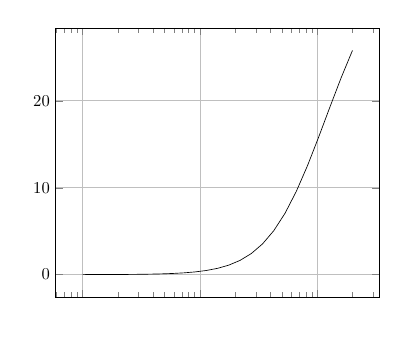
\begin{tikzpicture}[scale=0.6]
        \begin{semilogxaxis}[grid=major, xticklabel=\empty]
        \addplot [domain=1:200] {40*(1-(60*x+10000)/(x*x + 60*x+10000))};
        \end{semilogxaxis}
    \end{tikzpicture}
\end{minipage}
\hfill
\begin{minipage}{0.49\columnwidth}
    \centering \hspace{1em} Pole \\[0.5em]
    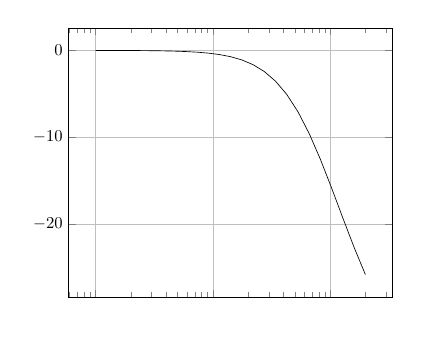
\begin{tikzpicture}[scale=0.6]
        \begin{semilogxaxis}[grid=major, xticklabel=\empty]
            \addplot[domain=1:200]  {40*((60*x+10000)/(x*x + 60*x+10000)-1)};
        \end{semilogxaxis}
    \end{tikzpicture}
\end{minipage}

\dotfill

\textit{1st Order Phase Response:} $\angle H(j\omega) = \pm \angle (1 + j \omega \tau) = \arctan(\omega \tau)$

Connect $\frac{1}{10\tau} < \omega < \frac{10}{\tau}$ w/ straight line.

\begin{table}[h!]
    \centering
    \begin{tabular}{lrr}
        \toprule
        & zero & pole \\
        \midrule
        $\omega \tau \leq 0.1$ & \SI{0}{\degree} & \SI{0}{\degree} \\
        $\omega \tau = 1$ & $+\SI{45}{\degree}$ & $-\SI{45}{\degree}$  \\
        $\omega \tau > 10$ & $+\SI{90}{\degree}$ & $-\SI{90}{\degree}$ \\
        $0.1 < \omega \tau < 10$ & $+\SI{45}{\degree/dec}$ & $-\SI{45}{\degree/dec}$ \\
        \bottomrule
    \end{tabular}
\end{table} \vspace{-.5em}

\begin{minipage}{0.49\columnwidth}
    \centering \hspace{1em} Zero \\[0.5em]
    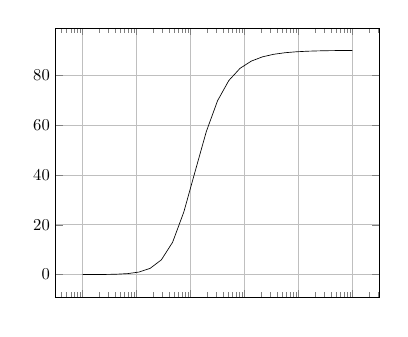
\begin{tikzpicture}[scale=0.6]
        \begin{semilogxaxis}[grid=major, xticklabel=\empty]
        \addplot [domain=1:100000] {90*(1-(60*x+10000)/(x*x + 60*x+10000))};
        \end{semilogxaxis}
    \end{tikzpicture}
\end{minipage}
\hfill
\begin{minipage}{0.49\columnwidth}
    \centering \hspace{1em} Pole \\[0.5em]
    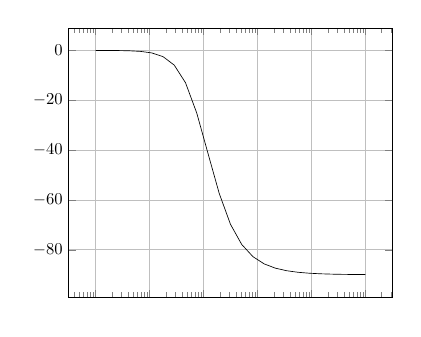
\begin{tikzpicture}[scale=0.6]
        \begin{semilogxaxis}[grid=major, xticklabel=\empty]
            \addplot[domain=1:100000]  {90*((60*x+10000)/(x*x + 60*x+10000)-1)};
        \end{semilogxaxis}
    \end{tikzpicture}
\end{minipage}

\dotfill

\textit{2nd Order Magnitude Response:} $H_{\text{dB}} = \pm 20 \log| 1 - (\omega \tau)^2 + j 2 \zeta (\omega \tau) |$

Standard form: $H(j\omega) = 1 + 2\zeta (j\omega\tau) + (j\omega\tau)^2$

$\quad s^2 + 2 \zeta \omega_0 s + \omega_0^2 = \left( \frac{s}{\omega_0} \right)^2 + 2 \zeta \left(\frac{s}{\omega_0}\right) + 1 = 0, \quad s = j\omega$

$\quad$Corner freq: $\omega_0 = 1/\tau \implies H_{\text{dB}} = \pm 20 \log(2\zeta)$

\begin{table}[h!]
    \centering
    \begin{tabular}{lrr}
        \toprule
        & Complex conj zeros & Complex conj poles \\
        \midrule
        $\omega \tau \ll 1$ & \SI{0}{dB} & \SI{0}{dB} \\
        $\omega \tau = 1$ & $20 \log 2 \zeta$ & $-20 \log 2 \zeta$ \\
        $\omega \tau \gg 1$ & $+\SI{40}{dB/dec}$ & $-\SI{40}{dB/dec}$  \\
        Btw regions & Depends on $\zeta$ & Depends on $\zeta$ \\
        \bottomrule
    \end{tabular}
\end{table} \vspace{-.5em}

\vspace{-.5em}
\dotfill

\textit{2nd Order Phase Response:} $\angle H(j\omega) = \arctan \left( \frac{2\zeta(\omega \tau)}{1 - (\omega \tau)^2} \right)$

\begin{table}[h!]
    \centering
    \begin{tabular}{lrr}
        \toprule
        & Complex conj zeros & Complex conj poles \\
        \midrule
        $\omega \tau \ll 1$ & \SI{0}{\degree} & \SI{0}{\degree} \\
        $\omega \tau = 1$ & $+\SI{90}{\degree}$ & $-\SI{90}{\degree}$ \\
        $\omega \tau \gg 1$ & $+\SI{180}{\degree}$ & $-\SI{180}{\degree}$  \\
        Btw regions & Depends on $\zeta$ & Depends on $\zeta$ \\
        \bottomrule
    \end{tabular}
\end{table}


\cleardoublepage


\textbf{Laplace Transforms}

$\mathcal{L}[f(t)] = \int_{0^-}^\infty f(t) e^{-st}\ dt = F(s)$

$\mathcal{L}^{-1}[F(s)] = \frac{1}{2\pi j} \int_{\sigma_1 - j\infty}^{\sigma_1 + j\infty} F(s) e^{st}\ ds = f(t)$

$\mathcal{L}[f'] = sF(s) - f(0)$ \hfill $\mathcal{L}[f''] = s^2 F(s) - sf(0) - f'(0)$

$\mathcal{L}[u(t)] = \frac{1}{s}$ \hfill $\mathcal{L}[u(t-t_0)] = \frac{e^{st_0}}{s}$ \hfill $\mathcal{L}[p(t)] = \frac{1-e^{st_0}}{s}$

$\mathcal{L}[\delta(t)] = 1$ \hfill $\mathcal{L}[\delta(t-t_0)] = e^{st_0}$

IVT: $\lim_{t \to 0^+} f(t) = \lim_{s \to \infty} sF(s)$ \hfill FVT: $\lim_{t \to \infty} = \lim_{s \to 0} sF(s)$

$\quad$Poles of $F(s)$ on LHS of $s$-plane (except poles at $s=0$)

\vspace{-.5em}
\dotfill

\textit{Partial Fraction Expansion}

Real \& distinct roots: $\frac{P(s)}{Q(s)} = \frac{K_1}{s+p_1} + \cdots + \frac{K_j}{s+p_j} + \cdots + \frac{K_n}{s + p_n}$

$\quad K_j = \frac{P(s)}{Q(s)} (s+p_j) |_{s=-p_j}$

$\quad \mathcal{L}^{-1} \left[  \frac{P(s)}{Q(s)}\right] = u(t) \left( K_1 e^{-p_1 t} + \cdots + K_j e^{-p_j t} + \cdots + K_n e^{-p_n t} \right)$

Distinct complex roots: $\frac{P(s)}{Q(s)} = \frac{K}{s + (\alpha - j\beta)} + \frac{K^*}{s + (\alpha + j\beta)} + \cdots$

$\quad K = \frac{P(s)}{Q(s)} (s + \alpha - j\beta) |_{s=-(\alpha - j\beta)} = |K| \angle \theta_K$

$\quad \mathcal{L}^{-1} \left[ \frac{P(s)}{Q(s)} \right] = u(t) \left[ 2|K| e^{-\alpha t} \cos(\beta t + \theta_K) + \cdots \right]$

Repeated real roots: $\frac{P(s)}{Q(s)} = \frac{K_1}{(s+p)^n} + \frac{K_2}{(s+p)^{n-1}} + \cdots + \frac{K_n}{s+p}$

$\quad K_j = \frac{1}{(j-1)!} \left[ \frac{d^{(j-1)}}{ds^{(j-1)}} (s+p)^n F(s) \right]_{s=-p}$

\dotfill

\textit{Laplace Domain Model of Inductor}

\begin{minipage}{0.6\columnwidth}
    $\mathcal{L} \{v_L(t)\} = V_L(s) = L[sI_L(s) - i_L(0^-)]$ \\[0.5em]
    $\mathcal{L} \{i_L(t)\} = I_L(s) = \frac{V_L(s)}{sL} + \frac{i_L(0^-)}{s}$
\end{minipage}
\begin{minipage}{0.39\columnwidth}
    \centering
    \begin{circuitikz}[american, scale=1.35]
        \ctikzset{bipoles/length=9mm}
        \draw (0, 0)
        to [short] (0.75, 0)
        to [L=$L$] (0.75, -1)
        to [short] (0, -1);
        % voltage label
        \draw (0.5, 0) to [short, -o] (0, 0);
        \draw (0.5, -1) to [short, -o] (0, -1);
        \draw (0, 0) to [open, v=$V_L(s)$] (0, -1);
    \end{circuitikz}
\end{minipage}

\begin{circuitikz}[american, scale=1.35]
    \ctikzset{bipoles/length=9mm}
    \draw (0, 0)
    to [short] (0.75, 0)
    to [L=$sL$] (0.75, -1)
    to [V=$Li_L(0^-$), invert] (0.75, -1.75)
    to [short] (0, -1.75);
    % voltage label
    \draw (0.5, 0) to [short, -o] (0, 0);
    \draw (0.5, -1.75) to [short, -o] (0, -1.75);
    \draw (0, 0) to [open, v=$V_L(s)$] (0, -1.75);
\end{circuitikz}
\hfill
\begin{circuitikz}[american, scale=1.35]
    \ctikzset{bipoles/length=9mm}
    \draw (0, 0)
    to [short] (0.75, 0)
    to [L=$sL$] (0.75, -1)
    to [short] (0, -1);
    \draw (0.75, 0)
    to [short] (1.5, 0)
    to [I, l=\mbox{$\frac{i_L(0^-)}{s}$}] (1.5, -1)
    to [short] (0.75, -1);
    % voltage label
    \draw (0.5, 0) to [short, -o] (0, 0);
    \draw (0.5, -1) to [short, -o] (0, -1);
    \draw (0, 0) to [open, v=$V_L(s)$] (0, -1);
\end{circuitikz}

\vspace{-.5em}
\dotfill

\textit{Laplace Domain Model of Capacitor}

\begin{minipage}{0.6\columnwidth}
    $\mathcal{L} \{i_C(t)\} = I_C(s) = C[sV_C(s) - v_C(0^-)]$ \\[0.5em]
    $\mathcal{L} \{v_C(t)\} = \frac{I_C(s)}{sC} + \frac{v_c(0^-)}{s}$
\end{minipage}
\hfill
\begin{minipage}{0.39\columnwidth}
    \centering
    \begin{circuitikz}[american, scale=1.35]
        \ctikzset{bipoles/length=9mm}
        \draw (0, 0)
        to [short] (0.75, 0)
        to [C=$C$] (0.75, -1)
        to [short] (0, -1);
        % voltage label
        \draw (0.5, 0) to [short, -o] (0, 0);
        \draw (0.5, -1) to [short, -o] (0, -1);
        \draw (0, 0) to [open, v=$V_C(s)$] (0, -1);
    \end{circuitikz}
\end{minipage}

\begin{circuitikz}[american, scale=1.35]
    \ctikzset{bipoles/length=9mm}
    \draw (0, 0)
    to [short] (0.75, 0)
    to [C=$\frac{1}{sC}$] (0.75, -1)
    to [V=$\frac{v_C(0^-)}{s}$] (0.75, -1.75)
    to [short] (0, -1.75);
    % voltage label
    \draw (0.5, 0) to [short, -o] (0, 0);
    \draw (0.5, -1.75) to [short, -o] (0, -1.75);
    \draw (0, 0) to [open, v=$V_C(s)$] (0, -1.75);
\end{circuitikz}
\hfill
\begin{circuitikz}[american, scale=1.35]
    \ctikzset{bipoles/length=9mm}
    \draw (0, 0)
    to [short] (0.65, 0)
    to [C=$\frac{1}{sC}$] (0.65, -1)
    to [short] (0, -1);
    \draw (0.65, 0)
    to [short] (1.65, 0)
    to [I, l=\mbox{$Cv_C(0^-)$}, invert] (1.65, -1)
    to [short] (0.65, -1);
    % voltage label
    \draw (0.5, 0) to [short, -o] (0, 0);
    \draw (0.5, -1) to [short, -o] (0, -1);
    \draw (0, 0) to [open, v=$V_C(s)$] (0, -1);
\end{circuitikz}


\newpage

\textbf{Impulse Response}

$Y(s) = H(s) X(s)$

$\quad x(t) = \delta(t) \implies \mathcal{L}[\delta(t)] = 1 \implies y(t) = \mathcal{L}^{-1}[H(s)] = h(t)$

$\quad$Given $h(t)$, $y(t) = \mathcal{L}^{-1} [\mathcal{L}[h(t)] \mathcal{L}[x(t)]]$

\dotfill

\begin{minipage}{0.4\columnwidth}
    \textbf{Op-Amps} \vspace{1em}

    \begin{circuitikz}[american, scale=1]
        \ctikzset{bipoles/length=10mm}
        \draw (0,0) node [above] {$v_{(-)}$} to[short, o-] ++(0.5,0)
        node[op amp, anchor=-] (OA) {};
        \draw (OA.+) to [short, -o] ++(-0.5, 0) node[above] {$v_{(+)}$};
        \draw (OA.out)
        to [short] ++(0.25, 0)
        to ++(0,-0.5) node[ground] {}
        ++(0.5, 0.65) to [open, v=$v_0$] ++(0, -1.25);
    \end{circuitikz}
\end{minipage}
\hfill
\begin{minipage}{0.59\columnwidth}
    \textit{Assumptions}
    \begin{enumerate}
        \item $i_{(+)}=i_{(-)} = 0$
        \item $v_{(+)} - v_{(-)} = 0$
        \item Gain $A \approx \infty \implies v_{(+)} = v_{(-)}$
        \item $\beta \approx \infty \implies A = \text{const}$
    \end{enumerate}
\end{minipage}

\dotfill

\textit{Inverting Amplifer}

\begin{minipage}{0.59\columnwidth}
    \begin{circuitikz}[american, scale=1]
        \ctikzset{bipoles/length=10mm}
        \draw (0, 0) node[op amp] (opamp) {};
        \draw (opamp.-) to [R, l_=$R_1$] (-2.9, 0.35) -- (-3, 0.35)
        to [V=$v_{\text{in}}$] (-3, -1)
        to (-3, -1) node[ground] {};

        \draw (opamp.-) to [short, *-] ++(0, 1) coordinate (leftC)
        to [R=$R_f$] (leftC -| opamp.out)
        to [short, -*] (opamp.out)
        to [short, -o] (1.5, 0)
        to (1.5, -1) node[ground] {};
        \draw (1.95, 0.275) to [open, v=$v_0$] (1.95, -1.5);

        \draw (opamp.+) to [short] ++(0, -0.65) node[ground] {};
    \end{circuitikz}
\end{minipage}
\hfill
\begin{minipage}{0.3\columnwidth}
    $\frac{v_0}{v_{\text{in}}} = -\frac{R_f}{R_1} = A_f$ \\[1em]
    $v_0 = A_f v_{\text{in}}$ \\[1em]
    $A_f$ called closed-loop (feedback) gain
\end{minipage}

\dotfill

\textit{Non-Inverting Amplifier}

\begin{minipage}{0.59\columnwidth}
    \begin{circuitikz}[american, scale=1]
        \ctikzset{bipoles/length=10mm}
        \draw (0, 0) node[op amp] (opamp) {};
        \draw (opamp.-) to [R, l_=$R_1$, i<=$i_{\text{in}}$, invert] (-2.9, 0.35) -- (-3, 0.35)
        to (-3, -1) node[ground] {};

        \draw (opamp.-) to [short, *-] ++(0, 1) coordinate (leftC)
        to [R=$R_f$] (leftC -| opamp.out)
        to [short, -*] (opamp.out)
        to [short, -o] (1.5, 0)
        to (1.5, -1) node[ground] {};
        \draw (1.95, 0.275) to [open, v=$v_0$] (1.95, -1.5);

        \draw (opamp.+)
        to [short] ++(-1, 0)
        to [V=$v_{\text{in}}$] ++(0, -1)
        node[ground, yshift=.5em] {};
    \end{circuitikz}
\end{minipage}
\hfill
\begin{minipage}{0.3\columnwidth}
    $\frac{0-v_{\text{in}}}{R_1} = \frac{v_{\text{in}} - v_0}{R_f}$ \\[1em]
    $\frac{v_0}{v_{\text{in}}} = 1+\frac{R_f}{R_1} = A_f$
\end{minipage}

\dotfill

\textit{Voltage Follower (Unity Gain Buffer)}

\begin{minipage}{0.5\columnwidth}
    \begin{circuitikz}[american, scale=1]
        \ctikzset{bipoles/length=10mm}
        \draw (0, 0) node[op amp] (opamp) {};

        \draw (opamp.-) to [short, -] ++(0, 1) coordinate (leftC)
        to [short] (leftC -| opamp.out)
        to [short, -*] (opamp.out)
        to [short, -o] (1.5, 0)
        to (1.5, -1) node[ground] {};
        \draw (1.95, 0.275) to [open, v=$v_0$] (1.95, -1.5);

        \draw (opamp.+)
        to [short] ++(-1, 0)
        to [V=$v_{\text{in}}$] ++(0, -1)
        node[ground, yshift=.5em] {};
    \end{circuitikz}
\end{minipage}
\hfill
\begin{minipage}{0.49\columnwidth}
    $R_f = \SI{0}{\ohm},\ R_1 \to \infty$ \\[1em]
    $v_0 = v_{\text{in}}$ \\[1em]
    $A_f = 1$
\end{minipage}

\dotfill

\textit{Summing Amplifier}

\begin{circuitikz}[american, scale=1]
    \ctikzset{bipoles/length=10mm}
    \draw (0, 0) node[op amp] (opamp) {};

    \draw (-0.8, 0.35)
    to [short, -*] (-1.25, 0.35)
    to [R, l_=$R_1$] (-3, 0.35)
    to [short=$v_1$, o-] ++(0, 0);
    \draw (-1.25, 0.35)
    to [short] (-1.25, -0.5)
    to [R, l_= $R_2$] (-3, -0.5)
    to [short=$v_2$, o-] ++(0, 0);
    \draw (-1.25, 0.35)
    to [short] (-1.25, -2)
    to [R, l_= $R_n$] (-3, -2)
    to [short=$v_n$, o-] ++(0, 0);

    \draw (-2.15, -1) node[] {$\vdots$};

    \draw (opamp.-) to [short, *-] ++(0, 1) coordinate (leftC)
    to [R=$R_f$] (leftC -| opamp.out)
    to [short, -*] (opamp.out)
    to [short, -o] (1.5, 0)
    to (1.5, -1) node[ground] {};
    \draw (1.95, 0.275) to [open, v=$v_0$] (1.95, -1.5);

    \draw (opamp.+) to [short] ++(0, -0.65) node[ground] {};
\end{circuitikz}

$\frac{v_1 - 0}{R} + \frac{v_n - 0}{R} + \cdots + \frac{v_n - 0}{R} = \frac{0-v_0}{R_f}$

$v_0 = -\frac{R_f}{R} (v_1 + v_2 + \cdots + v_n)$


\cleardoublepage


\textit{Difference Amplifier}

\begin{minipage}{0.59\columnwidth}
    \begin{circuitikz}[american, scale=1]
        \ctikzset{bipoles/length=10mm}
        \draw (0, 0) node[op amp] (opamp) {};

        \draw (opamp.-)
        to [short] ++(-1, 0)
        to [R, l_=$R$] ++(-1, 0)
        to [short=$v_1$, -o] ++(-0.5, 0);

        \draw (opamp.-) to [short, *-] ++(0, 1) coordinate (leftC)
        to [R=$R_f$] (leftC -| opamp.out)
        to [short, -*] (opamp.out)
        to [short, -o] (1.5, 0)
        to (1.5, -1) node[ground] {};
        \draw (1.95, 0.275) to [open, v=$v_0$] (1.95, -1.5);

        \draw (opamp.+)
        to [short] ++(-0.5, 0)
        to [R=$R$, *-] ++(0, -1)
        node[ground] {};
        \draw (opamp.+)
        to [short] ++(-1, 0)
        to [R=$R$] ++(-1, 0)
        to [short=$v_2$, -o] ++(-0.5, 0);
    \end{circuitikz}
\end{minipage}
\hfill
\begin{minipage}{0.3\columnwidth}
    $v_{(+)} = \frac{v_2}{2} = v_{(-)}$ \\[1em]
    $i_1 = \frac{v_1 - v_2/2}{R}$ \\[1em]
    $v_0 = \frac{v_2}{2} - i_1R$ \\[1em]
    $v_0 = v_2 - v_1$
\end{minipage}

\dotfill

\textit{Differentiator}

\begin{circuitikz}[american, scale=1]
    \ctikzset{bipoles/length=10mm}
    \draw (0, 0) node[op amp] (opamp) {};
    \draw (opamp.-) to [C, l_=$C$] (-2.9, 0.35) -- (-3, 0.35)
    to [V=$v_{\text{in}}$] (-3, -1)
    to (-3, -1) node[ground] {};

    \draw (opamp.-) to [short, *-] ++(0, 1) coordinate (leftC)
    to [R=$R_f$] (leftC -| opamp.out)
    to [short, -*] (opamp.out)
    to [short, -o] (1.5, 0)
    to (1.5, -1) node[ground] {};
    \draw (1.95, 0.275) to [open, v=$v_0$] (1.95, -1.5);

    \draw (opamp.+) to [short] ++(0, -0.65) node[ground] {};
\end{circuitikz}

$i_{\text{in}} = i_f = C\frac{dv_{\text{in}}}{dt} = \frac{0-v_0}{R_f} \implies v_0 = -R_f C\frac{dv_{\text{in}}}{dt}$

\dotfill

\textit{Integrator}

\begin{circuitikz}[american, scale=1]
    \ctikzset{bipoles/length=10mm}
    \draw (0, 0) node[op amp] (opamp) {};
    \draw (opamp.-) to [R, l_=$R$] (-2.9, 0.35) -- (-3, 0.35)
    to [V=$v_{\text{in}}$] (-3, -1)
    to (-3, -1) node[ground] {};

    \draw (opamp.-) to [short, *-] ++(0, 1) coordinate (leftC)
    to [C=$C$] (leftC -| opamp.out)
    to [short, -*] (opamp.out)
    to [short, -o] (1.5, 0)
    to (1.5, -1) node[ground] {};
    \draw (1.95, 0.275) to [open, v=$v_0$] (1.95, -1.5);

    \draw (opamp.+) to [short] ++(0, -0.65) node[ground] {};
\end{circuitikz}

$\frac{v_{\text{in}}}{R} = -C\frac{dv_0}{dt} \implies v_0 = -\frac{1}{RC} \int_0^t v_{\text{in}}(x)\ dx$

\dotfill

\textbf{Non-Ideal Op-Amps}

$\frac{v_0}{v_s} = \frac{1}{1 + \frac{R_i}{R_0 + AR_i}}$ \hfill $A \to \infty$ for ideal case ($v_0 / v_s = 1$)

$v_0 = A(v_{(+)} - v_{(-)}) = A \Delta v,\ i_{\text{in}} = \Delta v / R_i$

\vspace{-.5em}
\dotfill

\textit{Comparator}

\begin{minipage}{0.54\columnwidth}
    \begin{circuitikz}[american, scale=1]
        \ctikzset{bipoles/length=10mm}
        \draw (0, 0) node[op amp] (opamp) {};
        \draw (opamp.-)
        to [R, l_=$R$] ++(-1, 0)
        to [short=$v_1$, -o] ++(-0.5, 0);

        \draw (opamp.out)
        to [short, -o] (1.5, 0)
        to (1.5, -1) node[ground] {};
        \draw (1.95, 0.275) to [open, v=$v_0$] (1.95, -1.5);

        \draw (opamp.+)
        to [short] ++(-1, 0)
        to [V=$v_{\text{in}}$] ++(0, -1)
        node[ground, yshift=.5em] {};
    \end{circuitikz}
\end{minipage}
\hfill
\begin{minipage}{0.45\columnwidth}
    $v_0 = A(v_{\text{ref}} - v_{\text{in}})$ \\[1em]
    For $E^+$ and $E^-$ to op-amp, \\[1em]
    $v_{\text{ref}} > v_{\text{in}} \implies v_0 = E^+$ \\[1em]
    $v_{\text{ref}} < v_{\text{in}} \implies v_0 = E^-$
\end{minipage}

Since $A$ large, any diff in $v_{\text{ref}}$ and $v_{\text{in}}$ will drive o/p to saturation.

\vspace{-.5em}
\dotfill

\textbf{Diode}

\begin{minipage}{0.5\columnwidth}
\begin{circuitikz}[american, scale=1]
    \ctikzset{bipoles/length=10mm}
    \draw (0, 0)
    to [short, i=$i_d$] (0.5, 0)
    to [diode, l_=\mbox{$+\ v_d\ -$}] (1, 0)
    to [short] (1.5, 0);
\end{circuitikz}
\end{minipage}
\hfill
\begin{minipage}{0.49\columnwidth}
\hfill $i_D = I_S (e^{qv_0(t) / (nkT)} - 1)$
\end{minipage}

If $v<0$, diode acts as open circuit ($i=0$); diode is reverse-biased.

If $v>0$, diode acts as short circuit ($v=0$); diode is forward-biased.


\newpage


\textit{Half-Wave Voltage Rectifier}

\begin{minipage}{0.6\columnwidth}
\begin{circuitikz}[american, scale=1]
    \ctikzset{bipoles/length=10mm}
    \draw (0, -2)
    to [V=$v_{\text{in}}$, invert] (0, 0)
    to [R=$R$, i=$i_d$] (2, 0)
    to [diode, l_=\mbox{$+\ v_d\ -$}] (3.5, 0)
    to [C, l=\mbox{$v_0 $}] (3.5, -2)
    to [short] (0, -2);
\end{circuitikz}
\end{minipage}
\hfill
\begin{minipage}{0.39\columnwidth}
    Diode conducts when $v_d = v_{\text{in}} - v_0 > 0 \implies v_{\text{in}} > v_0$ \\[1em]
    $i_{\text{d, max}} = \frac{v_{\text{in,max}} - v_0}{R}$
\end{minipage}

\dotfill

\textit{Full-Wave Voltage Rectifier}

\begin{minipage}{0.6\columnwidth}
\begin{circuitikz}[american, scale=1]
    \ctikzset{bipoles/length=5mm}
    \draw (0, -2)
    to [sV, l=\mbox{$v(t)$}] ++(0, 2)
    to [short] ++(2, 0)
    to [diode=$D_1$] ++(1, -1)
    to [short] ++(1, 0)
    to [R=$R$, v=$v_0$] ++(0, -2)
    to [short] ++(-3, 0)
    to [short] ++(0, 2)
    to [diode=$D_3$, -*] ++(1, 1);
    \draw (1, -1)
    to [diode=$D_4$, *-] ++(1, -1)
    to [diode=$D_2$, *-*] ++(1, 1);
    \draw (2, -2)
    to [short] (0, -2);
\end{circuitikz}
\end{minipage}
\hfill
\begin{minipage}{0.39\columnwidth}
    $v(t) = V_m \sin \omega t$ \\[1em]
    $v_0 = \begin{cases}
        v_{\text{in}}, & v_{\text{in}} > 0 \\
        -v_{\text{in}}, & v_{\text{in}} < 0
    \end{cases}$
\end{minipage}

\dotfill

\textit{Diode Rectification w/ Capacitive O/P Filter}

\begin{circuitikz}[american, scale=1]
    \ctikzset{bipoles/length=5mm}
    \draw (0, -2)
    to [sV, l=\mbox{$v(t)$}] ++(0, 2)
    to [diode, v=$v_D$] ++(2, 0)
    to [C=$C$] ++(0, -2)
    to [short] ++(-2, 0);
    \draw (2, 0)
    to [short] ++(2, 0)
    to [R=$R$, v=$v_0$] ++(0, -2)
    to [short] ++(-2, 0);
\end{circuitikz}

\dotfill

\textit{Diodes as Logic Circuits}

\begin{minipage}{0.5\columnwidth}
    \centering OR gate \\[1em]

    \begin{circuitikz}[american, scale=1]
        \ctikzset{bipoles/length=5mm}
        \draw node at (0, 0) [left] {$v_a$};
        \draw (0, 0)
        to [diode, o-] (2, 0)
        to [short] (2, -3)
        to [R=$R$] (2, -4)
        to node[ground] {} ++(0,0);
        \draw (0, -1)
        to [diode, o-] (2, -1);
        \draw node at (0, -1) [left] {$v_b$};
        \draw node at (0, -2) [left] {$v_c$};
        \draw (0, -2)
        to [diode, o-] (2, -2);
        \draw (2, -1) to [short, -*] (2.5, -1)
        to node [right] {$v$} ++(0, 0);
    \end{circuitikz}
\end{minipage}
\hfill
\begin{minipage}{0.49\columnwidth}
    \centering AND gate \\[1em]

    \begin{circuitikz}[american, scale=1]
        \ctikzset{bipoles/length=5mm}
        \draw node at (0, 0) [above] {$\SI{5}{V}$};
        \draw (0, 0)
        to [R, o-] (0, -2)
        to [short] (0, -4);
        \draw (0, -2) to [diode, -o] (-2, -2) to node [left] {$v_a$} ++(0, 0);
        \draw (0, -3) to [diode, -o] (-2, -3) to node [left] {$v_b$} ++(0, 0);
        \draw (0, -4) to [diode, -o] (-2, -4) to node [left] {$v_b$} ++(0, 0);
        \draw (0, -3) to [short, -*] (0.5, -3)
        to node [right] {$v$} ++(0, 0);
    \end{circuitikz}
\end{minipage}

\dotfill

\textbf{Non-Ideal Diode Models}

Const-voltage model: $v_D = v_{\text{on}}$ in FB region

\vspace{-3.25em}\hfill\begin{circuitikz}[american, scale=1]
    \ctikzset{bipoles/length=8mm}
    \draw (0, 0)
    to [diode, o-] (1, 0)
    to [V=$v_{\text{on}}$, -o] (2, 0);
\end{circuitikz}

Src-resistor model: $v_D = v_{\text{on}} + i_D R_D$ in FB region

$\quad P = i v_D + i^2 R_D$

\vspace{-3.25em}\hfill\begin{circuitikz}[american, scale=1]
    \ctikzset{bipoles/length=10mm}
    \draw (0, 0)
    to [diode, o-] (1, 0)
    to [V=$v_{\text{on}}$, -] (2, 0)
    to [R=$R_D$, -o] (3, 0);
\end{circuitikz}

\vspace{-.5em}
\dotfill

\textit{Precision Half-Wave Rectifier}

\begin{circuitikz}[american, scale=1]
    \ctikzset{bipoles/length=10mm}
    \draw (0, 0) node[op amp] (opamp) {};
    \draw (opamp.-) to [R, l_=$R_1$] (-2.9, 0.35) -- (-3, 0.35)
    to [short=$v_1$, -o] ++(0, 0);

    \draw (opamp.-) to [short, *-] ++(0, 1) coordinate (leftC)
    to [diode=$D_2$] (leftC -| opamp.out)
    to [short, -*] (opamp.out)
    to [short] (1.5, 0)
    to [diode=$D_1$] ++(0.5, 0)
    to [short, -o] ++(1, 0)
    to node [right] {$v_0$} ++(0, 0);

    \draw (leftC)
    to [short] ++(0, 1)
    to [R=$R_2$] ++(3.25, 0)
    to [short, -*] ++(0, -2.35);

    \draw (opamp.+) to [short] ++(0, -0.65) node[ground] {};
\end{circuitikz}


\cleardoublepage


$v_1 > 0$: $D_1$ RB and $D_2$ FB $\implies v_0 = 0$ \hfill ($i$ to $v_0$ ground)

$v_1 < 0$: $D_1$ FB and $D_2$ RB $\implies v_0 = -\frac{R_2}{R_1} v_1$ \hfill ($i$ to $v_1$ ground)

\dotfill

\textit{LPF}

\begin{circuitikz}[american, scale=1]
    \ctikzset{bipoles/length=10mm}
    \draw (0, 0) node[op amp] (opamp) {};
    \draw (opamp.-) to [R, l_=$R_1$] (-2.9, 0.35) -- (-3, 0.35)
    to [short=$\overline V_i$, -o] ++(0, 0);

    \draw (opamp.-) to [short, *-] ++(0, 1) coordinate (leftC)
    to [R=$R_f$] (leftC -| opamp.out)
    to [short, -*] (opamp.out)
    to [short] (1.5, 0)
    to [short, -o] ++(1, 0)
    to node [right] {$\overline V_0$} ++(0, 0);

    \draw (leftC)
    to [short] ++(0, 1)
    to [C=$1/(j\omega C)$] ++(1.7, 0)
    to [short, -] ++(0, -1);

    \draw (opamp.+) to [short] ++(0, -0.65) node[ground] {};
\end{circuitikz}

$\frac{\overline V_0}{\overline V_i} = -\frac{R_f}{R_1} \left( \frac{1}{1+j\omega R_f C} \right)$

\dotfill

\textbf{Two Port Networks}

\centering
\begin{circuitikz}[american, scale=1]
    \node[draw, thick, text width=4em, align=center, inner ysep=1em] (A) at (0,0) {linear network};
    \draw ($(A.north west)!.25!(A.west)$) to[short, i<_=$\mathbf I_1$, -o] ++(-1,0)
          ($(A.south west)!.25!(A.west)$) to[short, -o] ++(-1,0)
          ($(A.north east)!.25!(A.east)$) to[short, i<=$\mathbf I_2$, -o] ++(1,0)
          ($(A.south east)!.25!(A.east)$) to[short, -o] ++(1,0);
    \draw (-1.5, 0.45) to [open, v=$\mathbf V_1$] (-1.5, -0.45);
    \draw (1.5, 0.45) to [open, v=$\mathbf V_2$] (1.5, -0.45);
\end{circuitikz}
\flushleft \vspace{-1em}

\vspace{-.5em}
\dotfill

\textit{Admittance Parameters}

\begin{minipage}{0.39\columnwidth}
    $\begin{bmatrix}
        \mathbf I_1 \\ \mathbf I_2
    \end{bmatrix} =
    \begin{bmatrix}
        \mathbf y_{11} & \mathbf y_{12} \\
        \mathbf y_{21} & \mathbf y_{22}
    \end{bmatrix}
    \begin{bmatrix}
        \mathbf V_1 \\ \mathbf V_2
    \end{bmatrix}$ \\[1em]
    All units in [S]
\end{minipage}
\hfill
\begin{minipage}{0.55\columnwidth}
    $\mathbf y_{11} = \frac{\mathbf I_1}{\mathbf V_1} \bigg|_{\mathbf V_2 = 0}$ \hfill $\mathbf y_{12} = \frac{\mathbf I_1}{\mathbf V_2} \bigg|_{\mathbf V_1 = 0}$

    $\mathbf y_{21} = \frac{\mathbf I_2}{\mathbf V_1} \bigg|_{\mathbf V_2 = 0}$ \hfill $\mathbf y_{22} = \frac{\mathbf I_2}{\mathbf V_2} \bigg|_{\mathbf V_1 = 0}$
\end{minipage}

$\mathbf I_1 = \mathbf y_{11} \mathbf V_1 + \mathbf y_{12} \mathbf V_2$

$\mathbf I_2 = \mathbf y_{21} \mathbf V_1 + \mathbf y_{22} \mathbf V_2$

Can also compute by finding currents using nodal analysis.

$\mathbf y_{11}$: short ciruit i/p admittance

$\mathbf y_{22}$: short ciruit o/p admittance

$\mathbf y_{12},\ \mathbf y_{21}$: short ciruit transfer admittance

\vspace{-.5em}
\dotfill

\textit{Impedance Parameters}

\begin{minipage}{0.39\columnwidth}
    $\begin{bmatrix}
        \mathbf V_1 \\ \mathbf V_2
    \end{bmatrix} =
    \begin{bmatrix}
        \mathbf z_{11} & \mathbf z_{12} \\
        \mathbf z_{21} & \mathbf z_{22}
    \end{bmatrix}
    \begin{bmatrix}
        \mathbf I_1 \\ \mathbf I_2
    \end{bmatrix}$ \\[1em]
    All units in [$\Omega$]
\end{minipage}
\hfill
\begin{minipage}{0.55\columnwidth}
    $\mathbf z_{11} = \frac{\mathbf V_1}{\mathbf I_1} \bigg|_{\mathbf I_2 = 0}$ \hfill $\mathbf z_{12} = \frac{\mathbf V_1}{\mathbf I_2} \bigg|_{\mathbf I_1 = 0}$

    $\mathbf z_{21} = \frac{\mathbf V_2}{\mathbf I_1} \bigg|_{\mathbf I_2 = 0}$ \hfill $\mathbf z_{22} = \frac{\mathbf V_2}{\mathbf I_2} \bigg|_{\mathbf I_1 = 0}$
\end{minipage}

$\mathbf V_1 = \mathbf z_{11} \mathbf I_1 + \mathbf z_{12} \mathbf I_2$

$\mathbf V_2 = \mathbf z_{21} \mathbf I_1 + \mathbf z_{22} \mathbf I_2$

$\mathbf z_{11}$: short ciruit i/p impedance

$\mathbf z_{22}$: short ciruit o/p impedance

$\mathbf z_{12},\ \mathbf z_{21}$: short ciruit transfer impedance


\newpage


\textit{Hybrid Parameters}

\begin{minipage}{0.39\columnwidth}
    $\begin{bmatrix}
        \mathbf V_1 \\ \mathbf I_2
    \end{bmatrix} =
    \begin{bmatrix}
        \mathbf h_{11} & \mathbf h_{12} \\
        \mathbf h_{21} & \mathbf h_{22}
    \end{bmatrix}
    \begin{bmatrix}
        \mathbf I_1 \\ \mathbf V_2
    \end{bmatrix}$
\end{minipage}
\hfill
\begin{minipage}{0.55\columnwidth}
    $\mathbf h_{11} = \frac{\mathbf V_1}{\mathbf I_1} \bigg|_{\mathbf V_2 = 0}$ \hfill $\mathbf h_{12} = \frac{\mathbf V_1}{\mathbf V_2} \bigg|_{\mathbf I_1 = 0}$

    $\mathbf h_{21} = \frac{\mathbf I_2}{\mathbf I_1} \bigg|_{\mathbf V_2 = 0}$ \hfill $\mathbf h_{22} = \frac{\mathbf I_2}{\mathbf V_2} \bigg|_{\mathbf I_1 = 0}$
\end{minipage}

$\mathbf V_1 = \mathbf h_{11} \mathbf I_1 + \mathbf h_{12} \mathbf V_2$

$\mathbf I_2 = \mathbf h_{21} \mathbf I_1 + \mathbf h_{22} \mathbf V_2$

$\mathbf h_{11}$: short circuit input impedance [$\Omega$]

$\mathbf h_{22}$: open circuit input admittance [S]


$\mathbf h_{12}$: open circuit input reverse $V$ gain [pu]

$\mathbf h_{21}$: short circuit forward $I$ gain [pu]

\vspace{-.5em}
\dotfill

\textit{Transmission (ABCD) Parameters}

\begin{minipage}{0.39\columnwidth}
    $\begin{bmatrix}
        \mathbf V_1 \\ \mathbf I_1
    \end{bmatrix} =
    \begin{bmatrix}
        \mathbf A & \mathbf B \\
        \mathbf C & \mathbf D
    \end{bmatrix}
    \begin{bmatrix}
        \mathbf V_2 \\ - \mathbf I_2
    \end{bmatrix}$
\end{minipage}
\hfill
\begin{minipage}{0.55\columnwidth}
    $\mathbf A = \frac{\mathbf V_1}{\mathbf V_2} \bigg|_{\mathbf I_2 = 0}$ \hfill $\mathbf B = -\frac{\mathbf V_1}{\mathbf I_2} \bigg|_{\mathbf V_2 = 0}$

    $\mathbf C = \frac{\mathbf I_1}{\mathbf V_2} \bigg|_{\mathbf I_2 = 0}$ \hfill $\mathbf D = \frac{\mathbf I_1}{\mathbf I_2} \bigg|_{\mathbf V_2 = 0}$
\end{minipage}

$\mathbf V_1 = \mathbf A \mathbf V_2 - \mathbf B \mathbf I_2$

$\mathbf I_1 = \mathbf C \mathbf V_2 - \mathbf D \mathbf I_2$

$\mathbf A$: open circuit $V$ ratio [pu]

$\mathbf B$: -ve short circuit transfer impedance [$\Omega$]

$\mathbf C$: open circuit transfer admittance [S]

$\mathbf D$: -ve short circuit $I$ ratio [pu]

\vspace{-.5em}
\dotfill

\textit{Cascading Two Port Networks}

Most conveniently modelled using ABCD parameters.

$\begin{bmatrix}
    \mathbf A & \mathbf B \\
    \mathbf C & \mathbf D
\end{bmatrix} =
\begin{bmatrix}
    \mathbf A_a & \mathbf B_a \\
    \mathbf C_a & \mathbf D_a
\end{bmatrix}
\begin{bmatrix}
    \mathbf A_b & \mathbf B_b \\
    \mathbf C_b & \mathbf D_b
\end{bmatrix}$

\vspace{-.5em}
\begin{figure}[h!]
    \centering
    \begin{circuitikz}[american, scale=1]
        \node[draw, thick, text width=2em, align=center, inner ysep=2em] (A) at (0,0) {$N_a$};
        \draw ($(A.north west)!.25!(A.west)$) to[short, i<_=$\mathbf I_{1a}$, -o] ++(-1,0)
              ($(A.south west)!.25!(A.west)$) to[short, -o] ++(-1,0)
              ($(A.north east)!.25!(A.east)$) to[short, i<=$\mathbf I_{2a}$, -] ++(1,0)
              ($(A.south east)!.25!(A.east)$) to[short, -] ++(1,0);
        \draw (-1.5, 0.45) to [open, v=$\mathbf V_{1a}$] (-1.5, -0.45);
        \draw (0.85, 0.45) to [open, v=$\mathbf V_{2a}$] (0.85, -0.45);
    
        \node[draw, thick, text width=2em, align=center, inner ysep=2em, right of=A, xshift=5.5em] (B) {$N_b$};
        \draw ($(B.north west)!.25!(B.west)$) to[short, i<_=$\mathbf I_{1b}$, -] ++(-1,0)
              ($(B.south west)!.25!(B.west)$) to[short, -] ++(-1,0)
              ($(B.north east)!.25!(B.east)$) to[short, i<=$\mathbf I_{2b}$, -o] ++(1,0)
              ($(B.south east)!.25!(B.east)$) to[short, -o] ++(1,0);
        \draw (2.1, 0.45) to [open, v=$\mathbf V_{1b}$] (2.1, -0.45);
        \draw (4.45, 0.45) to [open, v=$\mathbf V_{2b}$] (4.45, -0.45);
    \end{circuitikz}
\end{figure}

\vspace{-.5em}
\dotfill

\textit{Thevenin Equivalent System}

\begin{circuitikz}[american, scale=1]
    \ctikzset{bipoles/length=8mm}
    \node[draw, thick, text width=4em, align=center, inner ysep=2em] (A) at (0,0) {[Z]};
    \draw ($(A.north west)!.25!(A.west)$) to[short, i<_=$\mathbf I_1$, -o] ++(-1,0)
          ($(A.south west)!.25!(A.west)$) to[short, -o] ++(-1,0)
          ($(A.north east)!.25!(A.east)$) to[short, i<=$\mathbf I_2$, -o] ++(1,0)
          ($(A.south east)!.25!(A.east)$) to[short, -o] ++(1,0);
    \draw (-1.15, 0.45) to [open, v=$\mathbf V_1$] (-1.15, -0.45);
    \draw (1.5, 0.45) to [open, v=$\mathbf V_2$] (1.5, -0.45);
    % left side
    \draw ($(A.north west)!.25!(A.west)$) to[short, i<_=$\mathbf I_1$, -o] ++(-1,0)
    to [generic, a=$Z_s$] ++(-1.5, 0)
    to [V=$V_s$] ++(0, -1.24)
    to [short] ++(1.48, 0);
\end{circuitikz}

$\begin{cases}
    \mathbf V_1 = \mathbf I_1 \mathbf z_{11} + \mathbf I_2 \mathbf z_{12} \\
    \mathbf V_2 = \mathbf I_1 \mathbf z_{21} + \mathbf I_2 \mathbf z_{22} \\
    \mathbf V_s = \mathbf V_1 + \mathbf I_1 \mathbf z_s
\end{cases}$
\hfill
$\implies$
\hfill
$\mathbf I_1 = \frac{\mathbf V_s - \mathbf I_2 \mathbf z_{12}}{\mathbf z_s + \mathbf z_{11}}$

$\mathbf V_2 = \underbrace{\frac{\mathbf z_{21}}{\mathbf z_{11} + \mathbf z_s} \mathbf V_s}_{\mathbf V_{\text{th}}} + \underbrace{\left( \mathbf z_{22} - \frac{\mathbf z_{12} \mathbf z_{21}}{\mathbf z_{11} + \mathbf z_s} \right)}_{\mathbf z_{\text{th}}} \mathbf I_2$











\cleardoublepage


\onecolumn

\begin{table}[h!]
    \centering
    \textit{LT Properties} \\[1em]

    \begin{tabular}{lll}
        \toprule
        Operation & Time domain & Laplace domain \\
        \midrule
        Scaling & $f(at),\quad a \geq 0$ & $\frac{1}{a} F\left(\frac{s}{a}\right)$ \\[1em]
        Time convolution & $f_1(t) * f_2(t)$ & $F_1(s) F_2(s)$ \\[1em]
        Time differentiation & $\frac{df}{dt}$ & $sF(s) - f(0^-)$ \\[1em]
        & $\frac{d^2 f}{dt^2}$ & $s^2 F(s) - sf(0^-) - f'(0^-)$ \\[1em]
        & $\frac{d^3 f}{dt^2}$ & $s^3 F(s) - s^2 f(0^-) - sf'(0^-) - f''(0^-)$ \\[1em]
        Time integration & $\int_{0^-}^t f(x)\ dx$ & $\frac{1}{s} F(s)$ \\[1.5em]
        & $\int_{-\infty}^t f(x)\ dx$ & $\frac{1}{s} F(s) + \frac{1}{s} \int_{-\infty}^{0^-} f(t)\ dt$ \\[1.5em]
        Time shift & $f(t-t_0) u(t-t_0)$ & $F(s)e^{-st_0},\quad t_0 \geq 0$ \\[1em]
        Frequency shift & $f(t)e^{s_0t}$ & $F(s-s_0)$ \\[1em]
        Frequency differentiation & $-tf(t)$ & $\frac{dF(s)}{ds}$ \\[1em]
        Initial value thm & $f(0^+)$ & $\lim_{s\to\infty} sF(s)$ \\[1em]
        Final value thm & $\lim_{t\to\infty} f(t)$ & $\lim_{s\to 0} sF(s)$ \\[1em]
        & & (poles of $sF(s)$ in LHP) \\
        \bottomrule
    \end{tabular}
\end{table} \vspace{-.5em}

\vspace{-.5em}
\dotfill


\begin{table*}[h!]
    \centering
    \textit{Unilateral LT of Important Functions} \\[1em]

    \begin{tabular}{c| cc |c| cc}
        \toprule
        & $f(t)$ & $F(s)$ & & $f(t)$ & $F(s)$ \\
        \midrule
        1 & $\delta(t)$ & 1 & 7 & $t^n e^{\lambda t} u(t)$ & $\frac{n!}{(s-\lambda)^{n+1}}$ \\[1em]
        2 & $u(t)$ & $\frac{1}{s}$ & 8 & $\cos(bt) u(t)$ & $\frac{s}{s^2 + b^2}$ \\[1em]
        3 & $tu(t)$ & $\frac{1}{s^2}$ & 9 & $\sin(bt) u(t)$ & $\frac{b}{s^2+b^2}$ \\[1em]
        4 & $t^n u(t)$ & $\frac{n!}{s^{n+1}}$ & 10 & $e^{-at} \cos(bt) u(t)$ & $\frac{s+a}{(s+a)^2 + b^2}$ \\[1em]
        5 & $e^{\lambda t} u(t)$ & $\frac{1}{s-\lambda}$ & 11 & $e^{-at} \sin(bt) u(t)$ & $\frac{b}{(s+a)^2 + b^2}$ \\[1em]
        6 & $t e^{\lambda t} u(t)$ & $\frac{1}{(s-\lambda)^2}$ & \\[1em]
        \bottomrule
    \end{tabular}
\end{table*}


\cleardoublepage


\textit{Parameter Conversion}

$\Delta \equiv$ determinant

\begin{table}[h!]
    \centering
    \begin{tabular}{cccc}
        % row 1
        $\begin{bmatrix}
            \mathbf z_{11} & \mathbf z_{12} \\
            \mathbf z_{21} & \mathbf z_{22}
        \end{bmatrix}$ &
        $\frac{1}{\Delta Y} \begin{bmatrix}
            \mathbf y_{11} & -\mathbf y_{12} \\
            -\mathbf y_{21} & \mathbf y_{11}
        \end{bmatrix}$ &
        $\frac{1}{\mathbf C} \begin{bmatrix}
            \mathbf A & \Delta T \\
            \mathbf 1 & \mathbf D
        \end{bmatrix}$ &
        $ \frac{1}{\mathbf h_{22}} \begin{bmatrix}
            \Delta H & \mathbf h_{12} \\
            - \mathbf h_{21} & 1
        \end{bmatrix}$ \\[1.5em]
        \midrule
        % row 2
        $\frac{1}{\Delta Z} \begin{bmatrix}
            \mathbf z_{22} & -\mathbf z_{12} \\
            -\mathbf z_{21} & \mathbf z_{11}
        \end{bmatrix}$
        & $\begin{bmatrix}
            \mathbf y_{11} & \mathbf y_{12} \\
            \mathbf y_{21} & \mathbf y_{22}
        \end{bmatrix}$ &
        $\frac{1}{\mathbf B} \begin{bmatrix}
            \mathbf D & -\Delta T \\
            -1 & \mathbf A
        \end{bmatrix}$ &
        $\frac{1}{\mathbf h_{11}} \begin{bmatrix}
            1 & -\mathbf h_{12} \\
            \mathbf h_{21} & \Delta H
        \end{bmatrix}$ \\[1.5em]
        \midrule
        % row 3
        $\frac{1}{\mathbf z_{21}} \begin{bmatrix}
            \mathbf z_{11} & \Delta Z \\
            1 & \mathbf z_{22}
        \end{bmatrix}$ &
        $-\frac{1}{\mathbf y_{21}} \begin{bmatrix}
            \mathbf y_{22} & 1 \\
            \Delta Y & \mathbf y_{11}
        \end{bmatrix}$
        & $\begin{bmatrix}
            \mathbf A & \mathbf B \\
            \mathbf C & \mathbf D
        \end{bmatrix}$ &
        $-\frac{1}{\mathbf h_{21}} \begin{bmatrix}
            \Delta H & \mathbf h_{11} \\
            \mathbf h_{22} & 1
        \end{bmatrix}$ \\[1.5em]
        \midrule
        % row 4
        $\frac{1}{\mathbf z_{22}} \begin{bmatrix}
            \Delta Z & \mathbf z_{12} \\
            -\mathbf z_{21} & 1
        \end{bmatrix}$
        &
        $\frac{1}{\mathbf y_{11}} \begin{bmatrix}
            1 & -\mathbf y_{12} \\
            \mathbf y_{21} & \Delta Y
        \end{bmatrix}$
        &
        $\frac{1}{\mathbf D} \begin{bmatrix}
            \mathbf B & \Delta T \\
            -1 & \mathbf C
        \end{bmatrix}$
        & $\begin{bmatrix}
            \mathbf h_{11} & \mathbf h_{12} \\
            \mathbf h_{21} & \mathbf h_{22}
        \end{bmatrix}$
    \end{tabular}
\end{table}





\end{document}
